\documentclass[a4paper,12pt]{extarticle}

% Для поддержки русского языка
\usepackage[T2A]{fontenc}
\usepackage[utf8]{inputenc}
\usepackage[english, russian]{babel}

\usepackage{geometry} % Простой способ задавать поля
	\geometry{top=20mm}
	\geometry{bottom=20mm}
	\geometry{left=20mm}
	\geometry{right=20mm}

\usepackage{indentfirst} % Отступ первого абзаца

\usepackage{amsmath,amsfonts,amssymb,amsthm,mathtools} % Формулы
\usepackage{icomma} % "Умная" запятая: $0,2$ --- число, $0, 2$ --- перечисление

\usepackage{graphicx}  % Для вставки рисунков
\graphicspath{{images/}}

\usepackage{hyperref}
\hypersetup{
  unicode=true,
  colorlinks=true,
  linkcolor=blue,
  citecolor=teal,
  urlcolor=magenta
}
\usepackage{enumitem}
\usepackage{framed}
\usepackage{xcolor}
\definecolor{mygreen}{RGB}{0,160,0}

\author{Татаринова А.Г.}
\title{Лабораторная работа 2}
\date{\today}

\begin{document}

\maketitle

\text{Цель}: познакомиться с основами CSS и вёрстки.
\begin{itemize}
    \item Лабораторная работа сдается преподавателю лично студентом.
    \item В ходе сдачи лабораторной работы показывается написанный код и даются по нему комментарии.
\end{itemize}

Справочники:
\begin{itemize}
    \item Сайт \url{htmlbook.ru}
    \item Основы HTML5 и CSS3 \url{https://metanit.com/web/html5/}
\end{itemize}

\section{Задание}
Изучите примеры использования CSS по ссылкам ниже. Обращайте внимание на
применяемые свойства в стилях.
\begin{enumerate}
  \item Добавление подчеркивания к заголовку - \href{https://htmlbook.ru/faq/kak-dobavit-podcherkivanie-k-zagolovku}{ссылка}
  \item Добавление пунктирного подчеркивания к тексту - \href{https://htmlbook.ru/faq/kak-sdelat-punktirnoe-podcherkivanie-teksta}{ссылка}
  \item Альтернатива тегу \textbf{<font>} - \href{https://htmlbook.ru/faq/kak-mne-oboytis-bez-tega-font}{ссылка}
  \item Отображение тегов на веб-странице - \href{https://htmlbook.ru/faq/kak-otobrazit-tegi-na-veb-stranitse}{ссылка}
  \item Выравнивание текста по правому и левому краю - \href{https://htmlbook.ru/faq/kak-vyrovnyat-tekst-odnovremenno-po-pravomu-i-levomu-kra}{ссылка}
  \item Добавление цветной рамки вокруг текста - \href{https://htmlbook.ru/faq/kak-dobavit-vokrug-teksta-ramku-opredelennogo-tsveta}{ссылка}
  \item  Выделение строки с помощью блока с закруглениями - \href{https://htmlbook.ru/faq/kak-vydelit-stroku-s-pomoshchyu-bloka-s-zakrugleniyami}{ссылка}
  \item Добавление линии сбоку от текста - \href{https://htmlbook.ru/faq/kak-dobavit-liniyu-vozle-teksta}{ссылка}
  \item Выделение цветом фрагмента текста - \href{https://htmlbook.ru/faq/kak-vydelit-drugim-tsvetom-fragment-teksta}{ссылка}
  \item Изменение цвета первой буквы в абзацах - \href{https://htmlbook.ru/faq/khochu-izmenit-tsvet-pervoy-bukvy-v-kazhdom-abzatse}{ссылка}
  \item Добавление рамки к изображению - \href{https://htmlbook.ru/faq/kak-dobavit-ramku-k-izobrazheniyu}{ссылка}
  \item Добавление подписи под изображением - \href{https://htmlbook.ru/faq/kak-dobavit-podpis-pod-fotografiey}{ссылка}
  \item Удаление рамок вокруг изображений - \href{https://htmlbook.ru/faq/kak-ubrat-ramku-vokrug-izobrazheniy-ssylok}{ссылка}
  \item Выравнивание изображения по центру веб-страницы - \href{https://htmlbook.ru/faq/kak-vyrovnyat-fotografiyu-po-tsentru-veb-stranitsy}{ссылка}
  \item Размещение нескольких изображений рядом по горизонтали - \href{https://htmlbook.ru/faq/kak-razmestit-neskolko-kartinok-ryadom-po-gorizontali}{ссылка}
  \item Изменение цвета текста в списке - \href{https://htmlbook.ru/faq/kak-izmenit-tsvet-teksta-v-spiske}{ссылка}
  \item Использование картинки вместо маркера в списке - \href{https://htmlbook.ru/faq/kak-vmesto-simvola-markera-ispolzovat-kartinku}{ссылка}
  \item Горизонтальное размещение элементов в списке - \href{https://htmlbook.ru/faq/kak-razmestit-elementy-spiska-gorizontalno}{ссылка}
  \item Горизонтальное меню с наклоном - \href{https://htmlbook.ru/faq/kak-sdelat-gorizontalnoe-menyu-s-naklonom}{ссылка}
  \item  Вывод термина и определения в одну строку - \href{https://htmlbook.ru/faq/kak-vyvesti-termin-i-opredelenie-v-odnu-stroku}{ссылка}
\end{enumerate}


\section{Задание}

Используя руководства и знания, полученные при выполнении предыдущего задания, напишите страницу, содержащую описание технического устройства (компьютер, принтер, сканер, ноутбук, видеокарту, процессор).

Требования к странице:
\begin{enumerate}
  \item Заголовок страницы с названием устройства.
  \item Основное описание устройства.
  \item Изображение устройства с рамкой и подписью.
  \item Список характеристик устройства, размещенный горизонтально.
  \item Фрагмент текста, выделенный цветом.
  \item Скрытый блок с дополнительной информацией.
  \item Всплывающая подсказка при наведении на определенные элементы.
\end{enumerate}

\begin{figure}[!ht]
    \centering
    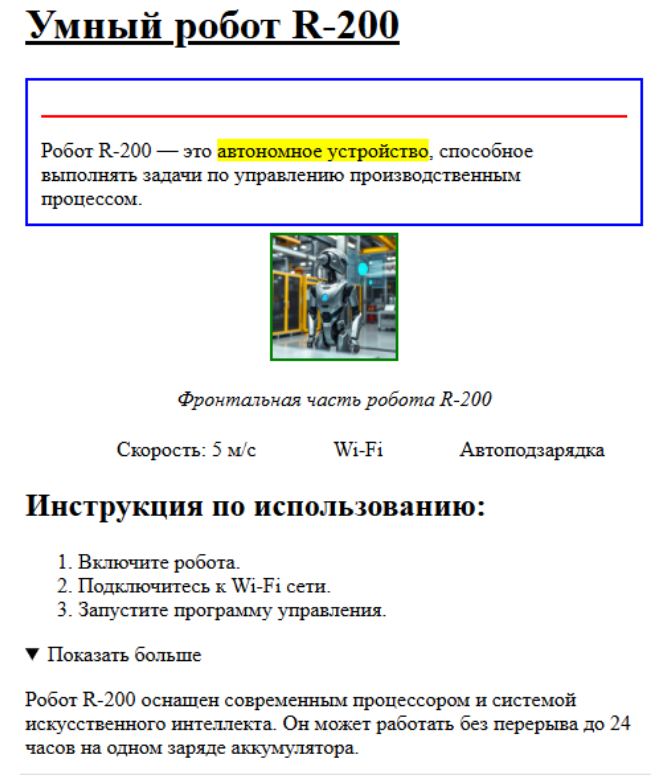
\includegraphics[width=0.4\textwidth]{lab2_task2.png}
\end{figure}

\section{Задание}
Дано следующее содержание веб-страницы
\begin{figure}[!ht]
    \centering
    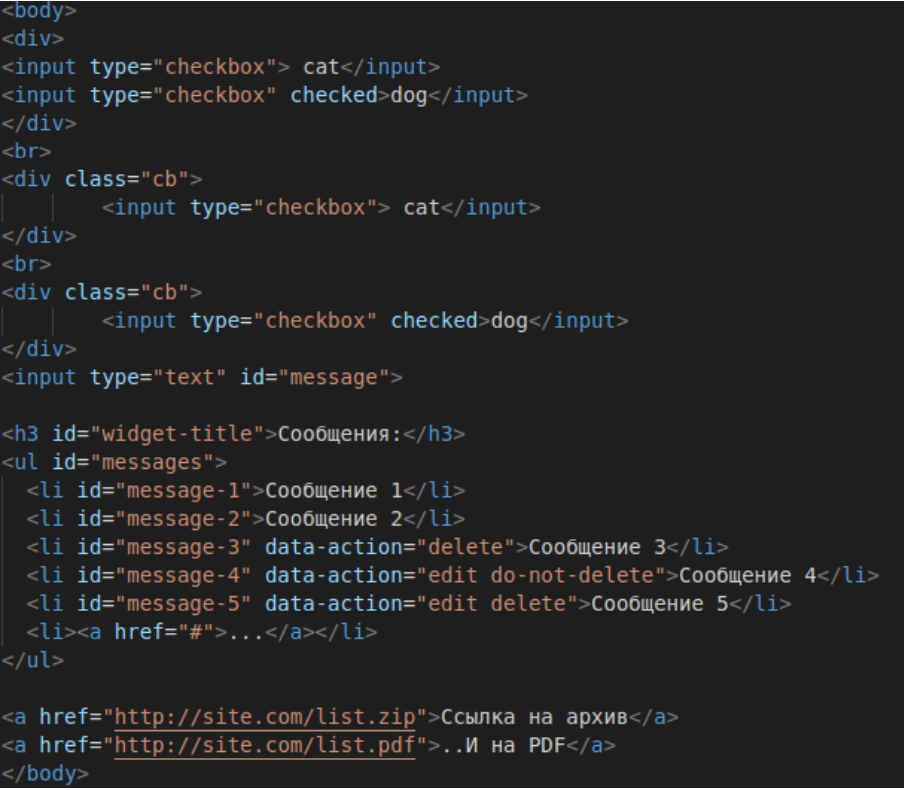
\includegraphics[width=0.9\textwidth]{lab2_task3.png}
\end{figure}

Задайте оформление элементов станицы через CSS-стили (\textbf{используйте нужные селекторы}) в
соответствии с заданиями, \textbf{не меняя html-код}:
\begin{enumerate}
  \item Выбрать элементы input типа checkbox и назначить им свойство box-shadow.
  \item Переопределить цвет тени box-shadow для отмеченных элементов checkbox.
  \item Задайте фоновый цвет для div-ов с классом cb.
  \item Найти все элементы с id=message и message-* и назначить им фоновый цвет.
  \item Найти все элементы с id=message-* и задайте им рамку и внешние поля.
  \item Найти все ссылки с расширением href="...zip" и задайте цвет ссылки при наведении на неё курсора мыши.
  \item Найти все элементы с атрибутом data-action, содержащим delete в списке (как полноценное слово, встречающееся с другими словами через пробел), и задайте цвет текста.
  \item Найти все элементы, у которых ЕСТЬ атрибут data-action, но НЕ содержащих delete в списке (как полноценное слово, встречающееся с другими через пробел), и задайте другой цвет фона.
  \item Выбрать все чётные элементы списка \#messages и изменить тип и ширину рамки.
  \item Выбрать один элемент сразу за заголовком h3\#widget-title на том же уровне вложенности, и сделать жирное начертание текста.
  \item Выбрать все ссылки, следующие за заголовком h3\#widget-title на том же уровне вложенности и сделать курсивное начертание текста.
  \item Выбрать ссылку внутри последнего элемента списка \#messages и назначить цвет ссылки при наведении на неё курсором мыши.
\end{enumerate}

\section{Задание}
Пройдите \href{https://flexboxfroggy.com/#ru}{обучающую игру} по возможностям Flexbox. В качестве отчета сохраните
скриншот о прохождении игры с указанием времени на скриншоте должны быть видны
стандартные часы ОС (сделайте скриншот всего рабочего стола)

\section{Задание}
Пройдите \href{https://cssgridgarden.com/#ru}{обучающую игру} по возможностям Grid. В качестве отчета сохраните
скриншот о прохождении игры с указанием времени на скриншоте должны быть видны
стандартные часы ОС (сделайте скриншот всего рабочего стола).

\section{Задание}
Создайте HTML-страницу с карточной сеткой товаров, используя технологию \textbf{Flexbox} для верстки. Также предусмотрите горизонтальное меню на странице и подвал со ссылками на контакты.

Пример страницы (с прокруткой):
\begin{figure}[!ht]
    \centering
    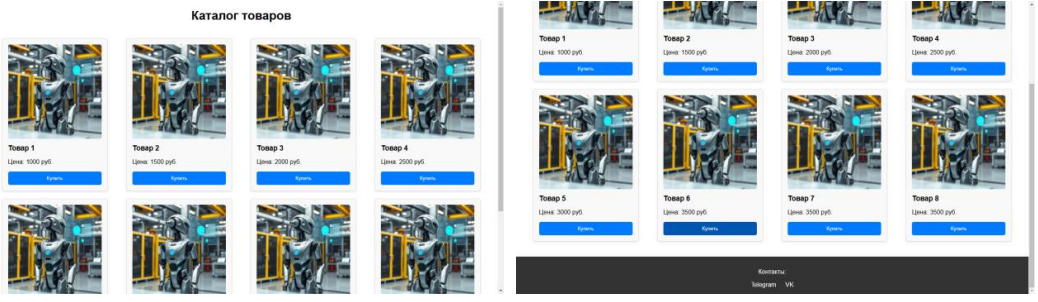
\includegraphics[width=0.9\textwidth]{lab2_task6.png}
\end{figure}

\section{Задание}
Создать HTML-страницу, представляющую собой информационный портал, используя технологию \textbf{CSS Grid} для верстки. 

Структура страницы должна быть следующей:
\begin{itemize}
  \item Шапка (header) с логотипом и навигацией.
  \item Главная секция (main), состоящая из:
  \begin{itemize}
    \item Боковой панели (sidebar) с категориями.
    \item Центральной области (content) с новостными статьями.
  \end{itemize}
  \item Подвал (footer) с контактной информацией.
\end{itemize}

Пример страницы:
\begin{figure}[!ht]
    \centering
    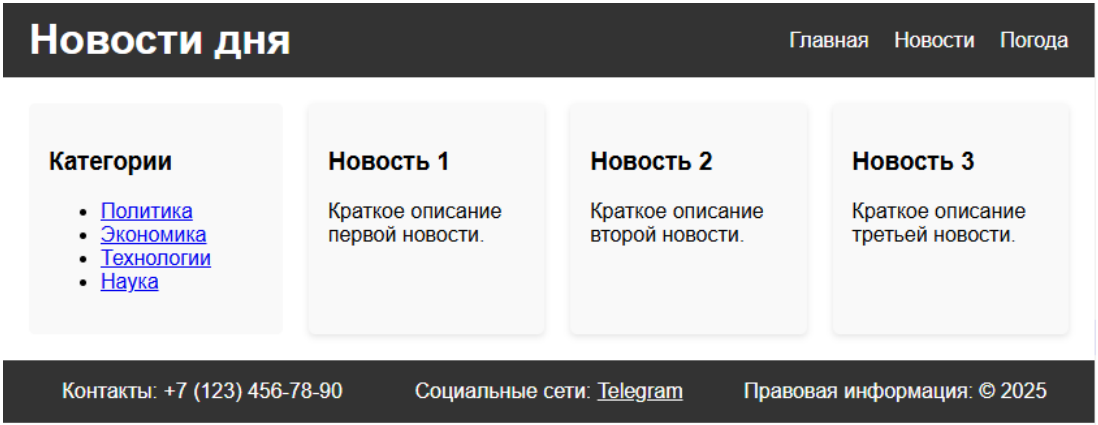
\includegraphics[width=0.9\textwidth]{lab2_task7.png}
\end{figure}

\section{Задание}
Оформите основные результаты своей курсовой работы с прошлых курсов в виде веб-страницы. Ориентируйтесь на представление своих результатов как представление вашего «стартапа».

\end{document}